\selectlanguage{english}
\chapter{The Standard Model and beyond}
\label{Chapter1}
%SourceDoc tesi.tex

Particle Physics studies the building blocks of the matter, the so called fundamental particle, and how they are governed by the four fundamental forces\footnote{In the thesis, Natural Units will be used: $c=\hbar=1$,  where $\hbar=h/2\pi=6.58211889(26)\cdot10^{-23}MeV s$ and $c=299792458~ms^{-1}$.}. \\
The best theory, explaining our  understanding of these particles and forces, is the \textit{Standard Model} (SM): developed during the 1970s, it has successfully explained almost all experimental results and precisely predicted a wide variety of physical phenomena. \\
This chapter will describe in details the Standard Model and some theories developed in order to solve some unanswered questions.

\section{The Standard Model}
\label{cap1:SM}
\subsection{Fundamental Particles}
\label{cap1:pi}
All matter around us is made of elementary particles with no substructure, well defined by some quantum numbers. These particles are divided into two groups: \textit{leptons}, with an entire value of electric charge, and \textit{quarks}, with a fractional charge. Each group consists of six particles, which are related in pairs or generations. The six quarks are paired in the three generations: the up and the down quark form the first generation (u, d), followed by the charm and strange  (c, s), then the top and bottom (or beauty) quark (t, b).  The six leptons are also similarly arranged in three generations: the electron (e) and the electronic neutrino ($\nu_{e}$), the muon ($\mu$)  with the muonic neutrino ($\nu_{\mu}$), and the tau ($\tau$) with the tauonic neutrino ($\nu_{\tau}$). While electron, muon and tau are charged particles, the neutrinos are electrically neutral. \tablename~\ref{leptonsSM} and \ref{quarkSM} summarise the features of leptons and quarks.
\begin{table}[ht]	
	\begin{center}
		\begin{tabular}{|ccc|}
			\hline     & \textbf{Leptons} &   \\
			\hline   Flavor & Charge & Mass[MeV]  \\
			\hline
			\hline
			electronic neutrino ($\nu_{e}$) & 0 & $<0.002$   \\
			electron ($e$) & -1 & 0.511   \\
			\hline
			muonic neutrino ($\nu_{\mu}$) & 0 & $<0.19$   \\
			muon ($\mu$) & -1 & 105.66   \\
			\hline
			tauonic neutrino ($\nu_{\tau}$) & 0 & $<18.2$ \\
			tau ($\tau$) & -1 & 1776.86$\pm$0.12  \\
			\hline
			\hline
		\end{tabular}
	\end{center}
	\caption{Standard Model leptons features \cite{PDG}.}
	\label{leptonsSM}
\end{table}

\begin{table}[htbp]	
	\begin{center}
		\begin{tabular}{|ccc|}
			\hline    & \textbf{Quark} &   \\
			\hline   Flavor & Carica & Massa[GeV]  \\
			\hline
			\hline
			up (\emph{u}) & +2/3 & 0.0022$^{+0.0006}_{-0.0004}$ \\   
			down (\emph{d}) & -1/3 & 0.0047$^{+0.0005}_{-0.0004}$ \\
			\hline
			charm (\emph{c}) & +2/3 & $1.28\pm3$ \\
			strange (\emph{s}) & -1/3 & $0.096\pm0.084$ \\
			\hline
			top (\emph{t}) & +2/3 & $173.1\pm0.6$ \\
			bottom (\emph{b}) & -1/3 & 4.18$^{+0.04}_{-0.03}$ \\   
			\hline
			\hline
		\end{tabular}
	\end{center}
	\caption{Standard Model quarks features \cite{PDG}.}
	\label{quarkSM}
\end{table}

Beside leptons and quarks, there are other particles called \textit{bosons} responsible of carrying (or mediating) the fundamental forces: Electromagnetic Force, responsible of all electrical and magnetic phenomena, is mediated by the photons {$\gamma$}; the Weak Force, responsible of some decays, is mediated by $W^{\pm}$ and $Z$ bosons; the Strong Force, responsible for example of the atomic structure, is mediated by the gluons ($g$). Last fundamental force, but not yet included in the SM due to its low strength compared to the others, is the Gravity, that is the weakest. \tablename~\ref{bosonsSM} summarises the features of the bosons.
\begin{table}[htbp]	
	\begin{center}
		\begin{tabular}{|cccc|}
			\hline    Bosons & Interaction & Charge & Mass[GeV]  \\
			\hline
			\hline
			 photon ($\gamma$) &  Electromagnetic & 0 & 0   \\
			 \hline
			 $W^{\pm}$ & Weak & $\pm$1 & 80.385$\pm$0.015   \\
			 \hline 
             	 	 $Z^{0}$ & Weak & 0 & 91.1876$\pm$0.0021   \\
			 \hline
			 gluoni & Strong & 0 & 0 \\
			\hline
			\hline
		\end{tabular}
	\end{center}
	\caption{Standard Model bosons features \cite{PDG}.}
	\label{bosonsSM}
\end{table}
\figurename~\ref{SM_zoo} shows the elementary particles described.
\begin{figure}[htbp]
\centering
%\includegraphics[width=0.45\textwidth]{Images/SM_zoo}
\includegraphics[width=0.45\textwidth]{Images/SM_zoo}
\caption{Elementary particles. }
\label{SM_zoo}
\end{figure}

\subsection{Gauge Symmetries}
\label{cap1:gaugeSymm}
The present belief is that all particles interactions may be dictated by the so called \textit{local gauge symmetries} and this is connected with the idea that  the conserved physical quantities (such as electric charge) are conserved in local regions of space and not just globally\cite{HalzenMartin}. \\
In particular, for the SM, the gauge group symmetry can be written as:
\[
SU(3)_{C}\otimes SU(2)_{L}\otimes U(1)_{Y}
\label{gaugeMS}
\]
where $SU(3)_{C}$ is the non-abelian group of strong interaction (QCD) and $SU(2)_{L}\otimes U(1)_{Y}$ is the group of the electroweak sector (EW) in which the electromagnetic and the weak force are described by one unified theory. As said, the SM is a local gauge theory and is it possible to associate a lagrangian obtained summing the contribution of the two gauge group:
\begin{equation}
\mathcal{L}_{MS} = \mathcal{L}_{EWK} + \mathcal{L}_{QCD}
\label{Lms}
\end{equation}

\begin{comment}
%The connection between symmetries and conservation laws is best discussed in the framework of Lagrangian Field Theory.\\
The fundamental quantity in classical mechanics is the action \textit{S}, the time integral of the Lagrangian \textit{L} (defined as the difference between the kinematic and potential energy):
\begin{equation}
S = \int L\, dt = \int \mathcal{L}(\phi, \partial \phi / \partial x_{\mu}) \,d^{4}x
\end{equation}
where $\mathcal{L}$ is the Lagrangian Density\footnote{however, following standard use in field theory, we will often refer to $\mathcal{L}$ simply Lagrangian.} 
and $\phi$ is the field, itself a function of the continuous parameters $x_{\mu}$ \cite{Peskin}\cite{Maggiore}. \\
Thanks to the \textit{Principle of least action}\footnote{Fixed the values of the coordinates at the initial and at the final time, classical trajectory which satisfies these conditions is an extremum of the action.} is possible deduce the particle equations of motion, the so called Euler-Lagrange equations (\ref{Eul_Lagr_Eq}):
\begin{equation}
\frac{\partial \mathcal{L}}{\partial \phi} - \frac{\partial}{\partial x_{\mu}}\frac{\partial \mathcal{L}}{\partial(\partial \phi / \partial x_{\mu})} = 0
\label{Eul_Lagr_Eq}
\end{equation}
%The relationship between symmetries and conservation laws is summarized in \textit{Noether's theorem}: 
\end{comment}

\subsubsection{QED}\index{QED}\label{QED}
%Quantum electrodynamics (QED) describes the interactions between photons and electrons. 
Starting point of the electroweak theory, is the  Quantum Electrodynamics, where is described the interaction of electron with photon.\\
Let's start with a complex field $\psi$ describing a free electron with mass m: its Lagrangian is
%Its motion is described by the Dirac Equation that follow from
% while the Dirac equation describes its motion. It can be shown Dirac equation follows from
\begin{equation}
\mathcal{L} = \bar{\psi}(i\gamma^{\mu}\partial_{\mu}-m)\psi
\label{L_electron}
\end{equation}
and its equation of motion can be deduced by the Dirac Equation.\\%, obtained substituting \ref{L_electron} in \ref{Eul_Lagr_Eq}. \\
The electromagnetic (em)  field instead is described by the four-vector gauge potential $A_{\mu}$. The field strength tensor is defined as:
\begin{equation}
F_{\mu\nu} = \partial_{\mu}A_{\nu} - \partial_{\nu}A_{\mu}
\label{F_em}
\end{equation}
and the equation of motion, in presence of an external current $J^{\mu}$ is:
\begin{equation}
\partial_{\mu}F^{\mu\nu} = QeJ^{\nu}
\label{Motion_em}
\end{equation}
In case now the electron interacts with the em field, the new Lagrangian is:
\begin{equation}
\mathcal{L}_{EM} = \bar{\psi}(i\gamma^{\mu}D_{\mu}-m)\psi - \frac{1}{4}F_{\mu\nu}F^{\mu\nu}
\label{L_electron_em}
\end{equation}
where $D_{\mu}$, known as covariant derivative, is defined as
\begin{equation}
D_{\mu} = \partial_{\mu} + ieQA_{\mu}
\label{D_covariante}
\end{equation}
and the last term in \ref{L_electron_em} stands for Maxwell's equation. \\
It can be shown that \ref{L_electron_em} is invariant under the phase transformation:
\begin{equation}
\psi(x)\to e^{-iQ\theta} \psi(x)
\label{global_trans}
\end{equation}
with $\theta \in \Re$. This transformation belongs to the group U(1) and according to Noether's theorem, it implies the existence of a conserved quantity: in this case, the electric charge.
Since once the value of $\theta$ is fixed, the invariance is specified for all space and time, it is known as \textit{global gauge invariance}. \\
More interesting is the case in which the parameter $\theta$ depends on space and time in a completely arbitrary way:
\begin{equation}
\psi(x)\to e^{-iQ\theta(x)} \psi(x)
\label{local_trans}
\end{equation}
and the Lagrangian \ref{L_electron_em} is not invariant.
It can be shown that, in oder to restore the Lagrangian invariance, the potential $A_{\mu}$ must satisfy following condition:
\begin{equation}
A_{\mu} \to A_{\mu} + \frac{1}{e}\partial_{\mu}\theta
\label{A_trans}
\end{equation}
Under \ref{local_trans} and \ref{A_trans} the Lagrangian \ref{L_electron_em} is invariant.\\ 
One can observe the absence of mass term in the Lagrangian: this means that the boson associated to the potential $A_{\mu}$, the photon, must be massless: the presence of a mass term would make the Lagrangian not invariant under gauge transformation. \\

\subsubsection{QCD}\index{QCD}\label{QCD}
The interaction between quarks and gluons is described by the Quantum Chromodynamics. \\
For quarks \cite{QCD}, it must be considered a new quantum number, the colour, such that each species of quark may have three different colours: $q_{j,\ j = 1, 2, 3}$ (red, green, blue). In order to avoid the existence of non-observed extra states with non-zero colour, one needs to further postulate that all asymptotic states are colourless, i.e. singlets under rotations in colour space. This assumption is known as the confinement hypothesis, because it implies the non-observability of free quarks: since quarks carry colour they are confined within colour-singlet bound states. \\
For free quark described by the field $q_{j}$, the Lagrangian is:
\begin{equation}
\mathcal{L} = \bar{q_{j}}(i\gamma^{\mu}\partial_{\mu} - m)q_{j}
\label{L_quark}
\end{equation}
In order to describe the  interaction between quarks and gluons, it is needed to change the quark derivative by covariant objects. Since there are now eight independent gauge parameters, eight different gauge bosons $G^{\mu}_{a}(x)$, the so-called gluons, are needed:
\begin{equation}
D^{\mu}_{q_{j}} \equiv [\partial^{\mu}- ig_{s}\frac{\lambda^{a}}{2}G^{\mu}_{a}(x)]
\label{D_covariante_qcd}
\end{equation}
The corresponding field strengths are also introduced:
\begin{equation}
G^{\mu\nu}_{a} = \partial^{\mu}G^{\nu}_{a} - \partial^{\nu}G^{\mu}_{a} + g_{s}f^{abc}G^{\mu}_{b}G^{\nu}_{c}
\label{G_munu}
\end{equation}
where $g_{s}$ is the coupling constant.
Hence, in case of interaction the new Lagrangian is:
\begin{equation}
\mathcal{L}_{QCD} = \bar{q_{j}}(i\gamma^{\mu}D_{\mu} - m)q_{j} -\frac{1}{4}G^{\mu\nu}_{a}G^{a}_{\mu\nu}
\label{L_quark_gluon}
\end{equation}
It can be shown \ref{L_quark_gluon} is invariant under arbitrary global $SU(3)_{C}$ transformations in colour space \ref{q_tranf_global}:
\begin{equation}
q(x) \to q'(x) = Uq(x) \equiv e^{i\theta_{a}T^{a}}q(x), \quad a = 1, 2, ...,8
\label{q_tranf_global}
\end{equation}
where $T_{a}$ are the generators of the SU(3) (a = $N^{2} - 1 = 3^{2} - 1 = 8)$ group linked with the $\lambda_{a}$ Gell-Mann matrices. \\
More interesting is the case in which $\theta$ depends on local coordinates, $\theta_{a}$ = $\theta_{a}$(x):
\begin{equation}
q(x) \to q'(x) = Uq(x) \equiv e^{i\theta_{a}(x)\frac{\lambda^{a}}{2}}q(x), \quad a = 1, 2, ...,8
\label{q_tranf_local}
\end{equation}
The group is non-Abelian since not all the generators $\lambda_{a}$ commute with each other. \\
To ensure the invariance of the Lagrangian \ref{L_quark_gluon}, the gauge fields must transform as follow:
\begin{equation}
G_{\mu a} \to G_{\mu a} - \frac{1}{g_{s}} \partial_{\mu}\theta_{a} - f_{abc}\theta^{b}G^{c}_{\mu}
\label{G_tranf_local}
\end{equation}
The field tensor $G^{\mu\nu}_{a}$ has a remarkable new property: imposing gauge symmetry (\ref{q_tranf_local} and \ref{G_tranf_local}), it has required kinematic energy term in \ref{L_quark_gluon} is not purely kinetic but includes an induced self-interaction between the gauge bosons. Decomposing the Lagrangian into its different pieces, there are three terms analogues to QED describing the free propagation of quarks and gluons and the quark-gluon interaction and two terms showing the presence of three and four gluon self-coupling in QCD reflecting the fact that gluons themselves carry color charge. They have no analogue in QED and arise on account of the non-Abelian character of the gauge group. As in QED, the absence of a mass term implies gluons must be massless.\\

\subsubsection{The electroweak theory}\index{EWK}
Low-energy experiments have provided a large amount of information about the dynamics underlying flavour-changing processes. The detailed analysis of the energy and angular distributions in $\beta$ decays, such as $\mu^{-} \to e^{-}\bar{\nu}_{e}\nu_{\mu}$, made clear that only the left-handed (right-handed) fermion (antifermion) chiralities participate in those weak transitions. Moreover, the strength of the interaction appears to be universal. \\
Using gauge invariance, it is possible to determine the right QED (\ref{L_electron_em}) and QCD (\ref{L_quark_gluon}) Lagrangians. To describe weak interactions, a more elaborated structure is needed, with several fermionic flavours and different properties for left- and right-handed fields. Moreover, the left-handed fermions should appear in doublets, and it would like to have gauge bosons in addition to the photon. The simplest group with doublet representations is SU(2) while to include also the electromagnetic interactions an additional U(1) group is needed. The obvious symmetry group to consider is then:
\begin{equation}
G \equiv SU(2)_{L} \otimes U(1)_{Y}
\label{EWK_group}
\end{equation}
where L refers to left-handed fields and Y stands for the weak hypercharge. \\
Let's consider a single family of leptons:
\begin{equation}
%\chi_L	&= \begin{pmatrix}\nu_{\emph{l}} \\\emph{l}^-\end{pmatrix}_L
\chi_{L} =  {\nu_{l} \choose l^{-}}_{L}, \quad \psi_{R} = l^{-}_{R}
\label{EWK_Singlet_doublet_Leptons}
\end{equation}
or for quarks
\begin{equation}
%\chi_L	&= \begin{pmatrix}\nu_{\emph{l}} \\\emph{l}^-\end{pmatrix}_L
\chi_{L} =  {u \choose d}_{L} , \quad \psi_{R} = u_{R},\ or\ d_{R}
\label{EWK_Singlet_doublet_Leptons}
\end{equation}
As in QED and QCD case, starts with free Lagrangian:
\begin{equation}
\mathcal{L} = i\bar{\chi}_{L}\gamma^{\mu}\partial_{\mu}\chi_{L} + i\bar{\psi}_{R}\gamma^{\mu}\partial_{\mu}\psi_{R}
\label{L0_EWK}
\end{equation}
The interaction is again introduced changing the derivative with the covariante:
\begin{equation}
D_{\mu} = \partial_{\mu} + igW_{\mu}^{a}T_{a} + ig'B_{\mu}Y
\label{D_EWK}
\end{equation}
where $W_{\mu}^{a}$ a = 1, 2, 3 are the three gauge bosons associated with the group $SU(2)_{L}$, $T^{a}$ its generators and g the coupling constants; $B_{\mu}$, Y and g are instead respectively the gauge boson, the generator and the coupling constant for the group $U(1)_{Y}$.
With $W_{\mu}^{a}$ and $B_{\mu}$ can be introduced also the tensor strength fields:
\begin{equation}
\begin{split}
W^{\mu\nu}_{a} &= \partial^{\mu}W^{\nu}_{a} - \partial^{\nu}W^{\mu}_{a} + g\epsilon^{abc}W^{\mu}_{b}W^{\nu}_{c} \\
B^{\mu\nu} 	 &= \partial^{\mu}B^{\nu} - \partial^{\nu}B^{\mu}
\label{WB_munu}
\end{split}
\end{equation}
Therefore, the properly Lagrangian is given by:
\begin{equation}
\mathcal{L} = i\bar{\chi}_{L}\gamma^{\mu}D_{\mu}\chi_{L} + i\bar{\psi}_{R}\gamma^{\mu}D_{\mu}\psi_{R} - \frac{1}{4}B_{\mu\nu}B^{\mu\nu} - \frac{1}{4}W_{\mu\nu}W^{\mu\nu}
\label{L_EWK}
\end{equation}
In \ref{L_EWK} $W_{\mu\nu} = W^{a}_{\mu\nu}\sigma^{a}/2$ with $\sigma^{a}$ 2x2 Pauli's matries. \\
As in QED and QCD case, also electroweak interaction is invariant under global transformation:
\begin{equation}
\begin{split}
\chi_{L} \to \chi_{L}' &= e^{i\alpha_{a} T^{a}  + i\beta Y} \chi_{L} \\
\psi_{R} \to \psi_{R}' &= e^{i\beta Y} \psi_{R} \\
\label{EWK_global}
\end{split}
\end{equation}
Moving to local transformation, in order to guarantee Lagrangian \ref{L_EWK} to be invariant, the gauge bosons must have following transformation rules:
\begin{equation}
\begin{split}
W^{a}_{\mu} &\to U_{L}(x) W^{a}_{\mu}  U_{L}(x)^{\dagger} - \frac{i}{g}\partial_{\mu}U_{L}(x) U_{L}(x)^{\dagger}, \\
B_{\mu} &\to B_{\mu} + \frac{1}{g'}\partial_{\mu}\beta
\label{EWK_global}
\end{split}
\end{equation}
where $U(x)_{L} = e^{i\sigma_{a} / 2\ \alpha(x)^{a}}$. The transformation of $B_{\mu}$ is identical to the one obtained in QED for the photon, while the $SU(2)_{L}\ W^{a}_{\mu}$ fields transform in analogous way to the gluon fields of QCD. \\
The gauge symmetry forbids to write a mass term for the gauge bosons in \ref{L_EWK}. Fermionic masses are also not possible, because they would communicate the left- and right-handed fields, which have different transformation properties, and therefore would produce an explicit breaking of the gauge symmetry. Thus, the $SU(2)_{L} \otimes U(1)_{Y}$ Lagrangian in \ref{L_EWK} only contains massless fields.\\
The term containing the $SU(2)_{L}$ matrix:
\begin{equation}
\frac{\sigma_{a}}{2}W_{\mu}^{a} = \frac{1}{\sqrt{2}}\begin{pmatrix} \sqrt{2}W^{3}_{\mu} & W_{\mu}^{+} \\ W_{\mu}^{-} & - \sqrt{2}W^{3}_{\mu} \end{pmatrix}
\end{equation}
gives rise to charged-current interactions with the bosons field $W_{\mu}^{\pm} \equiv (W^{1}_{\mu} \mp iW^{2}_{\mu}) / \sqrt{2}$. \\
La Lagrangian \ref{L_EWK}  contains also interactions with the neutral gauge field $W^{3}_{\mu}$ and $B_{\mu}$; one can define
\begin{equation}
Z_{\mu} = \frac{gW^{3}_{\mu} - g'B_{\mu}}	{\sqrt{g^{2}+g'{2}}}, \quad A_{\mu} = \frac{gW^{3}_{\mu} + g'B_{\mu}}	{\sqrt{g^{2}+g'{2}}}
\label{A_Z}
\end{equation}
and thinking them as a rotation, introducing the Weinberg angle $\theta_{W}$ so that $\cos\theta_{W} = g/{\sqrt{g^{2}+g'{2}}}$ (and $\sin\theta_{W} = g'/{\sqrt{g^{2}+g'{2}}}$):
\begin{equation}
Z_{\mu} = \cos\theta_{W}W^{3}_{\mu} - \sin\theta_{W}B_{\mu}, \quad A_{\mu} = \sin\theta_{W}W^{3}_{\mu} + \cos\theta_{W}B_{\mu}
\label{A_Z_2}
\end{equation}
or reversing:
\begin{equation}
{W^{3}_{\mu} \choose B_{\mu}} \equiv \begin{pmatrix} \cos\theta_{W} & \sin\theta_{W} \\ -\sin\theta_{W} & \cos\theta_{W} \end{pmatrix} {Z_{\mu} \choose A_{\mu}}
\label{W_B_A_Z}
\end{equation}
With these definitions, it can be observed the $A_{\mu}$ in \ref{L_EWK} couples in the same way with $l_{L}$ and $l_{R}$ as the photon: to get QED from these one needs to impose
\begin{equation}
g\sin\theta_{W} = g'\cos\theta_{W} = e
\label{g_gprime}
\end{equation}
At the same time, $Z_{\mu}$, can be identify with the Z boson, mediator of the Weak Interaction. \\
Once again, no mass term is present in \ref{L_EWK} and this means that $W^{\pm}$ and Z must be massless: this is in contrast with experimental evidence \cite{Wboson}\cite{Zboson}. \\
The way to generate the mass of the particle is through the so called \textit{Spontaneous Symmetry Breaking} (SSB): this mechanism appear in those cases where one has a symmetric Lagrangian, but a non-symmetric vacuum. 

\subsection{Spontaneous Symmetry Breaking: SSB}
Let's consider a complex scalar field $\phi(x) = (\phi_{1} + \phi_{2}) / \sqrt{2}$, with Lagrangian:
\begin{equation}
\mathcal{L} \equiv T - V = (\partial_{\mu}\phi)^{*}(\partial^{\mu}\phi) - \mu^{2}(\phi^{*}\phi)-\lambda(\phi^{*}\phi)^{2}
\label{L0}
\end{equation}
\ref{L0} is invariant under global phase transformation of the scalar field (it possesses a U(1) global gauge symmetry). \\
Considering the case when $\lambda > 0$, for the quadratic piece there are two possibilities:
\begin{itemize}
\item{$\mu^{2} > 0$:} the potential has only the trivial minimum $\phi = 0$
\item{$\mu^{2} < 0$:} the minimum is every point belonging to the circle (in the $\phi_{1}, \phi_{2}$) of radius $\nu$ such that:
	\begin{equation}
	(\phi_{1})^{2}+(\phi_{2})^{2} = \nu^{2} \quad with\ \nu^{2} = - \frac{\mu^{2}}{\lambda}
	\end{equation}
	as shown in \figurename~\ref{V_phi_potential}
\end{itemize}
\begin{figure}[htbp]
\centering
\includegraphics[width=0.45\textwidth]{Images/Vphi.png}
\caption{The potential $V(\phi)$ for a complex scalar field with $\lambda > 0$ and $\mu^{2} < 0$. }
\label{V_phi_potential}
\end{figure}
Owing to the U(1) phase-invariance of the Lagrangian \ref{L0}, there is an infinite number of degenerate states of minimum energy. 
By choosing a particular solution, $\phi_{1} = \nu$ and $\phi_{2} = 0$, as the ground state, the symmetry gets spontaneously broken. Parametrising the excitations over the ground state as:
\begin{equation}
\phi(x) \equiv \frac{1}{\sqrt{2}}[\nu+\eta(x)+i\xi(x)]
\label{phi_expansion}
\end{equation}
and substituting into \ref{L0}, one obtains:
\begin{equation}
\mathcal{L'} = \frac{1}{2}(\partial_{\mu}\xi)^{2} + \frac{1}{2}(\partial_{\mu}\eta)^{2} + \mu^{2}\eta^{2} + const. + O(\eta^{3})+O(\xi^{3})
\label{L0_prime}
\end{equation}
The third term has the form of a mass term for $\eta$-field: the $\eta$-mass is $m_{\eta} = \sqrt{-2\mu^{2}}$. The first term in \ref{L0_prime} represents the kinetic energy of the $\xi$-field but there is no corresponding mass term for the $\xi$. The fact there are massless excitations associated with the SSB mechanism is completely general result, known as the \textit{Goldstone theorem}: if a Lagrangian is invariant under a continuous symmetry group G, but the vacuum is only invariant under a subgroup $H\subset G$, then there must exist as many massless spin-0 particles (Goldstone bosons) as broken generators (i.e., generators of G which do not belong to H).

\subsubsection{Brout-Englert-Higgs mechanism}%: U(1) local gauge symmetry}
Let's move to consider the case for spontaneous breaking of U(1) local gauge symmetry.\\
Taking into account the covariant derivative \ref{D_covariante} where the gauge filed transforms as in \ref{A_trans}, the new Lagrangian can be written as
\begin{equation}
\mathcal{L} = D^{\mu}\phi^{*}D_{\mu}\phi -\mu^{2}\phi^{*}\phi-\lambda(\phi^{*}\phi)^{2}-\frac{1}{4}F_{\mu\nu}F^{\mu\nu}
\label{L0_U1}
\end{equation}
If $\mu^{2} > 0$, \ref{L0_U1} is just the QED Lagrangian for a charged scalar particle of mass $\mu$.
For the case $\mu^{2} < 0$, it is interesting to note that to lowest order in $\xi$, \ref{phi_expansion} can be expressed as
\begin{equation}
\phi(x) \equiv \frac{1}{\sqrt{2}}[\nu+\eta(x)]e^{i\xi(x)/\nu}
\label{phi_expansion_2}
\end{equation}
and this suggests to use different set of real field: h, $\theta$, $A_{\mu}$ where now
\begin{equation}
\begin{split}
\phi(x) &\to \frac{1}{\sqrt{2}}[\nu+h(x)]e^{i\theta(x)/\nu}, \\
A_{\mu} &\to A_{\mu}+ \frac{1}{e\nu}\partial_{\mu}\theta
\end{split}
\label{new_phi_A}
\end{equation}
This is a particular choice of gauge, with $\theta(x)$ chosen so that h is real. Substituting \ref{new_phi_A} in \ref{L0_U1}, one obtains:
\begin{equation}
\begin{split}
\mathcal{L}' = &\frac{1}{2}(\partial_{\mu}h)^{2}-\lambda\nu^{2}h^{2}+\frac{1}{2}e^{2}\nu^{2}A_{\mu}^{2}-\lambda\nu h^{3}-\frac{1}{4}\lambda h^{4}\\
&+\frac{1}{2}e^{2}A_{\mu}^{2}h^{2}+\nu e^{2}A_{\mu}^{2}h-\frac{1}{4}F_{\mu\nu}F^{\mu\nu}
\end{split}
\label{L0_U1_prime}
\end{equation}
The Goldstone boson does not appear in the theory: this is because it corresponds only to the degree of freedom to make a gauge transformation. The Lagrangian \ref{L0_U1_prime} describes just two interacting massive particles, a vector gauge bosoon $A_{\mu}$ and a massive scalar h, which is called a \textit{Higgs particle}. 
%This is called the \textit{Higgs mechanism}.\\
%\subsubsection{The Higgs Mechanism for $SU(2)_{L} \otimes U(1)_{Y}$ symmetry
Consider now the case of  $SU(2)_{L} \otimes U(1)_{Y}$ symmetry \cite{SU2_Hmechanism} with the Lagrangian
\begin{equation}
\mathcal{L} = (D_{\mu}\phi)^{\dagger}(D^{\mu}\phi)-\mu^{2}\phi^{\dagger}\phi-\lambda(\phi^{\dagger}\phi)^{2}
\label{L0_SU2}
\end{equation}
$D_{\mu}$ is the covariant derivative \ref{D_EWK} and $\phi$ is an SU(2) doublet of complex scalar fields:
\begin{equation}
\phi(x) \equiv {\phi^{+}(x) \choose \phi^0(x)}
\label{phi_SU2}
\end{equation}
\ref{L0_SU2} is invariant under local $SU(2)_{L} \otimes U(1)_{Y}$ transformations. \\
In $\mu^{2} < 0$ and $\lambda^{2} > 0$ conditions, to generate gauge boson masses, a vacuum expectation value of $\phi(x)$ must be chosen:
\begin{equation}
\phi_{0} \equiv \frac{1}{\sqrt{2}}{0 \choose \nu}
\label{SU2_U1_V0}
\end{equation}
In this way, the symmetry is broken and this generates a mass for the corresponding gauge boson. This particular choice of $\phi_{0}$ breaks both $SU(2)$ and $U(1)_{Y}$ gauge symmetries but since it is neutral, the $U(1)_{em}$ remains unbroken and this means the photon remains massless. \\
Now, substituting the vacuum expectation value $\phi_{0}$ for $\phi(x)$ in the Lagrangian \ref{L0_SU2}, the expression for W and Z bosons mass are:
\begin{equation}
M_{W}^{2} = \frac{\nu^{2}g^{2}}{4}, \quad M_{Z}^{2} = \frac{\nu^{2}g^{2}}{4\cos^{2}\theta_{W}}=\frac{M_{W}^{2}}{\cos^{2}{\theta_{W}}}
\label{WZ_mass_expression}
\end{equation}
From experimental observation \cite{PDG}:
\begin{equation}
M_{Z} = 91.1876\pm0.0021\ GeV, \quad M_{W} = 80.385\pm 0.015\ GeV
\end{equation}
From these experimental numbers, one obtains the electroweak mixing angle:
\begin{equation}
\sin^{2}\theta_{W} = 1-\frac{M^{2}_{W}}{M^{2}_{Z}} = 0.22336 \pm 0.00010
\end{equation}
The scalar vacuum expectation value is:
\begin{equation}
\nu=(\sqrt{2}G_{F})^{-1/2}=246\ GeV
\end{equation}
where $G_{F} = 1.1663787 \times 10^{-5} GeV^{-1}$ is the Fermi coupling whose value can be measured with the muon lifetime \cite{muLifetime}.\\
From \ref{L0_SU2}, the potential $V(\phi)$ can be seen as:
\begin{equation}
V(\phi)=-\frac{1}{4}\lambda\nu^{2}+V_{H}+V_{HG^{2}}
\label{V0_Higgs}
\end{equation}
The first term stands for mass of the new Higgs boson: $m_{H} = \sqrt{2\lambda\nu^{2}}$; the second represents Higgs boson self-interaction and the last the coupling with the weak bosons (W and Z). \\
It is interesting to note the same Higgs doublet which generates weak bosons masses can give masses also to leptons and quarks. \\
In particular, let's consider the following Lagrangian:
\begin{equation}
\mathcal{L} = -G_{e} [(\bar{\nu}_{e},\ \bar{e})_{L}{\phi^{+} \choose \phi^{0}}e_{R}+\bar{e}_{R}(\phi^{-},\ \bar{\phi}^{0}){\nu_{e} \choose e}_{L} ]
\label{L0_fermion_quark_mass}
\end{equation}
Substituting the expression of $\phi$:
\begin{equation}
\phi = \frac{1}{\sqrt{2}}{0 \choose \nu+h(x)}
\end{equation}
into \ref{L0_fermion_quark_mass}, the Lagrangian becomes:
\begin{equation}
\mathcal{L} = -\frac{G_{e}}{\sqrt{2}}\nu(\bar{e}_{L}e_{R}+\bar{e}_{R}e_{L})-\frac{G_{e}}{\sqrt{2}}h(\bar{e}_{L}e_{R}+\bar{e}_{R}e_{L})
% [(\bar{\nu}_{e},\ \bar{e})_{L}{\phi^{+} \choose \phi^{0}}e_{R}+\bar{e}_{R}(\phi^{-},\ \bar{\phi}^{0}){\nu_{e} \choose e}_{L} ]
\label{L0_fermion_quark_mass_2}
\end{equation}
Choosing $G_{e}$ so that $m_{e} = G_{e}\nu/\sqrt{2}$, since the $G_{e}$ is arbitrary, the actual mass of the electron is not predicted. \\
The quark masses are generated in the same way with the difference that to generate a mass for the upper member of a quark doublet, a new Higgs doublet from $\phi$ must be used:
\begin{equation}
\phi_{c} = i\tau\phi^{*}={-\bar{\phi}^{0} \choose \phi^{-}} \xrightarrow[breaking]{}\frac{1}{\sqrt{2}}{\nu+h(x) \choose 0}
\end{equation}
The new Lagrangian can be written as:
\begin{equation}
\mathcal{L}= -G_{d}(\bar{u}, \ \bar{d})_{L}{\phi^{+} \choose \phi^{0}}d_{R}-G_{u}(\bar{u}, \ \bar{d})_{L}{-\bar{\phi}^{0} \choose \phi^{-}}u_{R}\ +\ hermitian\  coniugate
\label{L0_quark_mass}
\end{equation}
In \ref{L0_quark_mass}, the (u,\ d) quark doublet are considered even if the weak interactions operate on $(u,\  d')_{L}$ where the primed states are  linear combinations of the flavour eigenstates\footnote{Linear combination of the flavour eigenstates considering Cabibbo-Kobayashi-Maswaka (CKM) matrix: $d'_i = \sum_{n=1}^NV_{in}d_n  $ where N = 3 is the number of quarks, $V_{in}$ is CKM matrix and $d_{n}$ are the d type quarks d, s, b.}. Using these new doublets, \ref{L0_quark_mass} is therefore of the form:
\begin{equation}
\mathcal{L}= -G_{d}^{ij}(\bar{u}, \ \bar{d}')_{L}{\phi^{+} \choose \phi^{0}}d_{jR}-G_{u}^{ij}(\bar{u}, \ \bar{d}')_{L}{-\bar{\phi}^{0} \choose \phi^{-}}u_{jR}\ +\ hermitian\  coniugate
\label{L0_quark_mass_2}
\end{equation}
with i, j = 1, ..., N,  where N is the number of quark doublet. Substituting $\phi_{c}$ expression, the masses depend on the arbitrary couplings $G_{u,d}$ but, as for electron, it cannot be predicted.\\
The choose of a particular single Higgs doublet is sufficient on one hand to generate the masses of both the gauge bosons and the fermions but on the other hand, the masses of the fermoins are just parameteres of the theory and are not predicted. 
%At the same time, the mass of the Higgs $m_{h}$ is itself not predicted: from the first two terms of the effective potential, $V(\phi) = \mu^{2}\phi^{\dagger}\phi+\lambda(\phi^{\dagger}\phi)^{2}+O(3)$, the mass can be defined as $m_{h}^{2} = 2\nu^{2}\lambda$: theoretical limits indicate that $m_{h} \ge 10\ GeV$. \\
\\ To summarise, the complete Lagrangian of the SM is:
\begin{equation}
\begin{split}
\mathcal{L}_{SM} &= \frac{1}{4}W_{\mu\nu}\cdot W^{\mu\nu} - \frac{1}{4}B_{\mu\nu}B^{\mu\nu} + \bar{L}\gamma^{\mu}(i\partial_{\mu}-g\frac{1}{2}\tau \cdot W_{\mu} -g'\frac{Y}{2}B_{\mu})L \\
&+\bar{R}\gamma^{\mu}(i\partial_{\mu}-g'\frac{Y}{2}B_{\mu})R+|i\partial_{\mu}-g\frac{1}{2}\tau \cdot W_{\mu} -g'\frac{Y}{2}B_{\mu}|^{2} -V{\phi} \\
&-(G_{1}\bar{L}\phi R+G_{2}\bar{L} \phi_{c}R +\ hermitian\ conjugate)
\label{L0_SM}
\end{split}
\end{equation}
The first two terms represent the $W^{\pm}$, Z, $\gamma$ kinetic energies and the self-interactions; the third and the fourth term the lepton and quark kinetic energies and their interaction with weak W, Z and $\gamma$; the last terms stand for masses and coupling of the Higgs, bosons, leptons and quark. \\
Without the Higgs boson, the calculability of the SM would have been spoiled. In particular, perturbative unitarity \cite{PerturbativeHiggs_1, PerturbativeHiggs_2} would be lost at high energies as the longitudinal W/Z boson scattering amplitude would grow as the centre-of-mass energy increases. Moreover, the radiative corrections to the gauge boson self-energies would exhibit dangerous logarithmic divergences that would be difficult to reconcile with Electroweak precision data. With the discovery of the Higgs boson, it has been experimentally established that the SM is based on a gauge theory that could a priori be consistently extrapolated to the Planck scale.

\section{The Higgs boson}
The SM Higgs boson is a CP-even scalar of spin 0 \cite{PDG}. Its mass is given by $m_{h} = \sqrt{2\lambda\nu^{2}}$, where $\lambda$ is the Higgs self-coupling parameter in the potential $V(\phi)$. The experimentally Higgs mass, $m_{h} \simeq 125\ GeV$ \cite{ALTAS_H, CMS_H}, implies $\lambda \simeq 0.1$. 
%Once the mass is know, in the SM, the boson width is very precisely predicted: for a mass of 125 GeV, the Higgs boson has a very narrow width of 4.2MeV.
The Higgs boson couplings to the fundamental particles are set by their masses: very weak for light particles, such as up and down quarks, and electrons, but strong for heavy particles such as the W and Z bosons and the top quark. In particular, the SM Higgs coupling to fundamental fermions are linearly proportional to the fermion masses $m_{f}$ ($y_{f} = m_{f}/\nu$ where $y_{f}$ is the Yukawa coupling) whereas the couplings to bosons are proportional to the squares of the boson masses. As consequence, the dominant mechanism for Higgs boson production and decay involve the coupling of H to W, Z and/or the third generation quarks and leptons. The Higgs boson coupling to  gluons is induced at leading order by a one-loop process in which H couples to a virtual $t\bar{t}$ pair. Likewise, the Higgs boson couplings to photons is also generated via loops, although in this case the one-loop graph with a virtual $W^{+}W^{-}$ pair provides the dominant contribution and the one involving a virtual $t\bar{t}$ pair is subdominant. \\

\subsection{The Higgs boson: production mechanisms}
The main production mechanisms at the LHC are gluon fusion, weak-boson fusion, associated production with gauge boson and associated production with a pair of top/antitop quarks. 
The corresponding Feynman diagrams are reported in \figurename~\ref{Feynman_H_production}; \figurename~\ref{plot_13tev_H_production} summarises the cross section as a function of Higgs mass for these dominant Higgs production processes for a center of mass energy of 13 TeV. 

\begin{figure}[htbp]
\centering
\includegraphics[width=0.45\textwidth]{Images/Feynman_H_production}
\caption{Main Leading Order Feynman diagrams contributing to the Higgs production: (a) gluon fusion, (b) Vector-boson fusion, (c) Higgs-strahlung (or associated production with a gauge boson), (d) associated production with a pair of top (or bottom quarks), (e-f) production in association with a single top quark.}
\label{Feynman_H_production}
\end{figure}
\begin{figure}[htbp]
\centering
\includegraphics[width=0.45\textwidth]{Images/plot_13tev_H_production}
\caption{Standard Model Higgs boson production cross section at $\sqrt{s} = 13\ TeV$ as a function of Higgs boson mass \cite{HiggsTWiki}.}
\label{plot_13tev_H_production}
\end{figure}

\subsubsection{Production mechanism: gluon fusion}
The Higgs boson production mechanism with the largest cross section is the gluon-fusion process: $gg \to H + X$, mediated by the exchange of a virtual, heavy top quark (\figurename~\ref{Feynman_H_production}a). Contributions from lighter quarks propagating in the loop are suppressed proportional to $m_{q}^{2}$. QCD radiative corrections to this process are also very important. At the LHC, with a $\sqrt{s} = 13\ TeV$, the value for the production cross section at the next-to next- to next  to leading order is \cite{ggF_value}:
\begin{equation}
\sigma^{N3LO}_{ggF} = 48.6pb^{+2.2pb(+4.6\%)}_{-3.3pb(+6.7\%)}(theory) \pm 1.6(3.2\%)(PDF+\alpha_{s})
\label{ggH_cross_section}
\end{equation}

\subsubsection{Production mechanism: Weak-boson fusion}
The SM Higgs production mode with the second-largest cross section is Vector Boson Fusion (VBF): $qq \to qqH$ (\figurename~\ref{Feynman_H_production}b). This mechanism proceeds by the scattering of two (anti-)quarks, mediated by exchange of a W or Z boson, with the Higgs boson radiated off the weak-boson propagator. The scattered quarks give rise to two hard jets in the forward and backward regions of the detector. Gluon radiation in the central-rapidity is suppressed thanks to the color-singlet nature of the weak-gauge boson exchange: this feature let to distinguish VBF from overwhelming QCD backgrounds including gluon-fusion induced Higgs + 2 jets production and production of H in association with a W or Z boson hadronically decaying. This process receive contributions at NLO from QCD and EW; QCD also contributes at NNLO.

\subsubsection{Production mechanism: Higgs-strahlung}
The next most relevant Higgs boson production mechanism is the Higgs-strahlung, the production of the Higgs boson with W or Z gauge bosons: $pp \to VH + X$ with $V = W^{\pm},Z$ (\figurename~\ref{Feynman_H_production}c). As in VBF, at NLO EW and QCD (due to corrections to the Drell-Yan cross section) give their contributions to this cross section. In addition, Higgs-strahlung receives non Drell-Yan-like corrections in the $q\bar{q}$ channel where the Higgs is radiated off top-quarks loops.

\subsubsection{Production mechanism: $t\bar{t}H$}
Higgs radiation off top quarks (\figurename~\ref{Feynman_H_production}d), $pp \to t\bar{t}H$, provides a direct probe of the top-Higgs Yukawa coupling. On the 10th April 2018, CMS announced the observation of the production of the Higgs boson together with a top-quark pair \cite{ttH}. \figurename~\ref{ttH} shows a possible t$\bar{t}$H event.
\begin{figure}[htbp]
\centering
\includegraphics[width=0.45\textwidth]{Images/ttH}
\caption{An event candidate for the production of a top quark and top anti-quark pair in conjunction with a Higgs Boson in the CMS detector. The Higgs decays into a $\tau^+$ lepton and a $\tau^-$ lepton; the $\tau^+$ in turn decays into hadrons and the $\tau^-$ decays into an electron. The decay product symbols are in blue. The top quark decays into three jets (sprays of lighter particles) whose names are given in purple. One of these is initiated by a b-quark. The top anti-quark decays into a muon and b-jet, whose names appear in red \cite{ttH_event}.}
\label{ttH}
\end{figure}

\subsection{The Higgs boson: decay channels}
As reported in \figurename~\ref{Higgs_decay}, the dominant decay modes for the Higgs boson are $H \to b\bar{b}$, $H \to WW^{*}$ followed by $H \to \gamma \gamma$, $H \to \tau^{+}\tau^{-}$ and $H \to ZZ^{*}$;  \tablename~\ref{Higgs_decay_table} summarises the branching ratios and the relative uncertainty for these decay channels. As example, in \figurename~\ref{Higgs_decay} is reported the mass 4 leptons mass distribution comparing data and simulation.\\
Of particular interest is the dimuon decay channel: it has a small branching ratio ($2.18 \times 10^{-4}$) but it plays a fundamental role. This decay channel is the only way to directly measure the Higgs-muon Yukawa coupling strength and the comparison of the cross section of $H\to \mu\mu$ and $H\to \tau\tau$ could provide constraints on the proportionality of the Higgs couplings to fermions of different generations and of leptons with different masses. 
\begin{figure}[htbp]
\centering
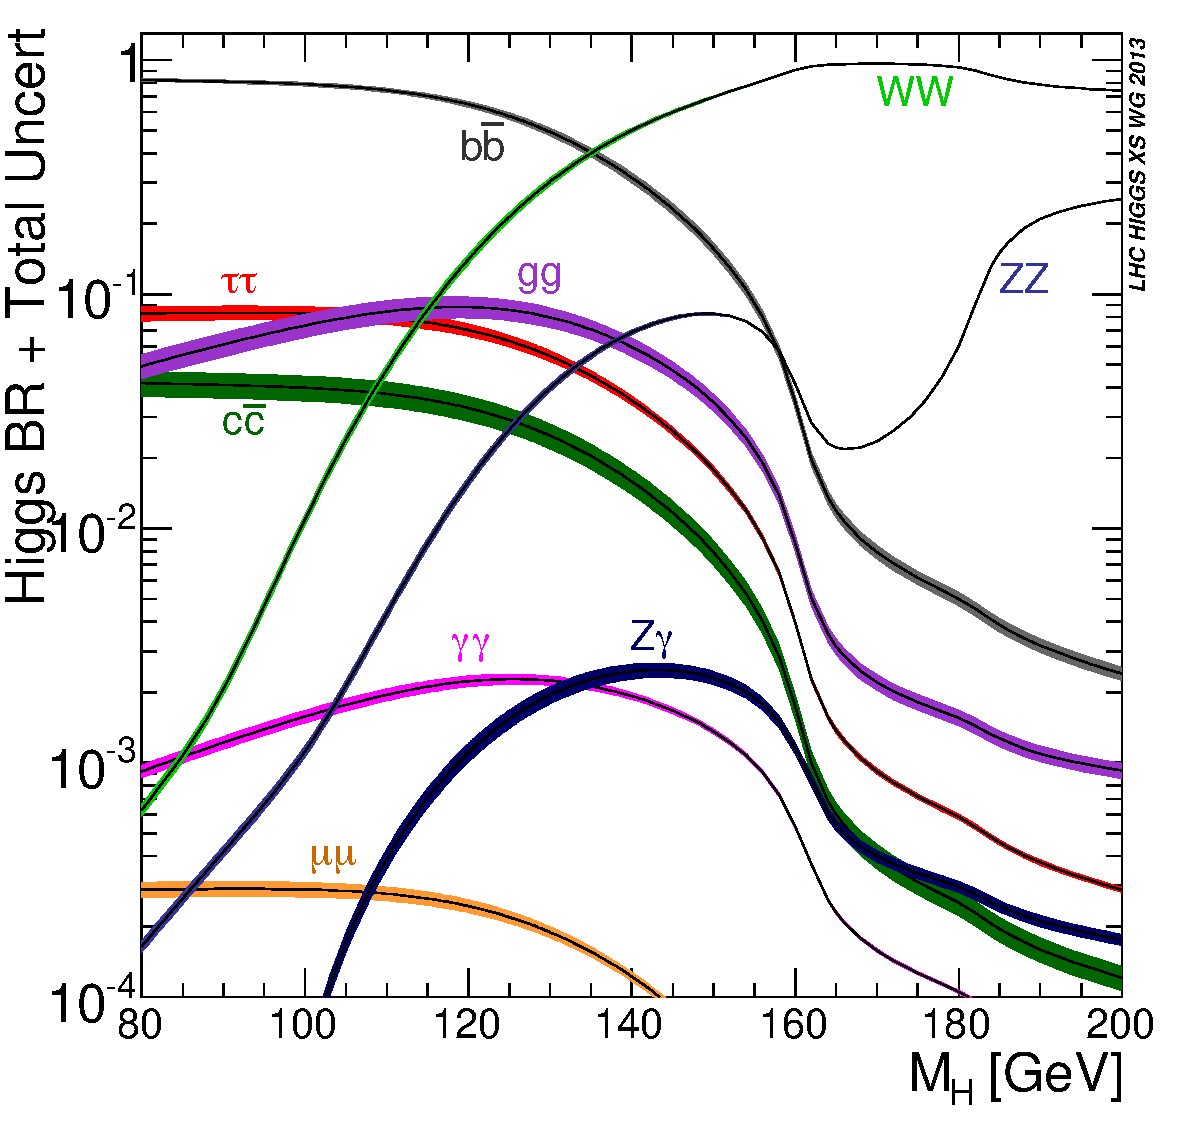
\includegraphics[width=0.45\textwidth]{Images/Higgs_decay}
\caption{Standard Model Higgs boson production cross section at $\sqrt{s} = 13\ TeV$ as a function of Higgs boson mass \cite{HiggsTWiki}.}
\label{Higgs_decay}
\end{figure}
\begin{table}[ht]	
	\begin{center}
		\begin{tabular}{ccc}
			\hline   Decay channel & Branching ratio  & Rel. uncertainty  \\
			\hline
			 \multirow{2}*{$H \to b\bar{b}$} & 			\multirow{2}*{$5.84 \times 10^{-1}$} &	 +3.2\% \\  &  & -3.3\% \\
			 \multirow{2}*{$H \to WW^{*}$} &			 \multirow{2}*{$2.14 \times 10^{-1}$} &	 +4.3\% \\  &  & -4.2\% \\
			 \multirow{2}*{$H \to \tau^{+}\tau^{-}$} &		 \multirow{2}*{$6.27 \times 10^{-2}$} &	 +5.7\% \\  &  & -5.7\% \\
			 \multirow{2}*{$H \to ZZ^{*}$} &				 \multirow{2}*{$2.62 \times 10^{-2}$} &	 +4.3\% \\  &  & -4.1\% \\
			 \multirow{2}*{$H \to \gamma \gamma$} & 	\multirow{2}*{$2.27 \times 10^{-3}$} &	 +5.0\% \\  &  & -4.9\% \\
			 \multirow{2}*{$H \to \mu \mu$} &			 \multirow{2}*{$2.18 \times 10^{-4}$} &	 +6.0\% \\  &  & -5.9\% \\
			\hline
		\end{tabular}
	\end{center}
	\caption{Branching ratio for a Higgs boson with $m_H$ = 125 GeV at 13 TeV \cite{BR_1, BR_2}.}
	\label{Higgs_decay_table}
\end{table}
\begin{figure}[htbp]
\centering
\includegraphics[width=0.5\textwidth]{Images/HZZ}
\caption{Distribution of the four-lepton reconstructed invariant mass $m_{4l}$ in the full mass range combining 2016 and 2017. Points with error bars represent the data and stacked histograms represent expected distributions of the signal and background processes \cite{HZZ_mass}}
\label{HZZ}
\end{figure}

\subsection{Latest Higgs results}
\subsubsection{Signal Strength}
In \figurename~\ref{SignalStrength} are reported the fit to the signal strength modifiers $\mu_i$: $\mu_i$ is defined as the ratio between the measured Higgs boson yield and its SM expectation. For a specific production and decay channel $i \to H \to f$ , the signal strengths for the production, $\mu_i$ , and for the decay, $\mu_f$ , are defined as,
\[
\mu_i = \frac{\sigma_i}{(\sigma_i)_{SM}},\ \ \ \mu^f = \frac{BR^f}{{BR}^f_{SM}}
\]
where $\sigma_i$ is the production cross section for $i \to H$ and $\mu^f$ is the the branching ratio for  $H \to f$; the "SM" refers to their respective SM predictions, so by definition, the SM corresponds to $\mu_i = \mu^f = 1$. Since $\sigma_i$ and $BR^f$ cannot be separately measured without additional assumptions, only the product of $\mu_i$ and $\mu^f $ can be extracted experimentally, leading to a signal strength $\mu^f_i$ for the combined production and decay:
\[
\mu^f_i = \frac{\sigma_i \cdot BR^f}{(\sigma_i)_{SM}\cdot {BR}^f_{SM}} = \mu_i \times \mu^f
\]
The combined measurement of the common signal strength modifier is \cite{LatestHiggsCMS}
\[
\mu = 1.17^{+0.06}_{-0.06}(stat.)^{+0.06}_{-0.05}(sig.th.)^{+0.06}_{-0.06}(other\ syst.) 
\]
\begin{figure}[htbp]
\centering
\includegraphics[width=0.45\textwidth]{Images/MuI}
\includegraphics[width=0.54\textwidth]{Images/MuF}
\includegraphics[width=0.45\textwidth]{Images/MuIeMuF}
\caption{Summary plot of the fit to the per-production mode (left) and per-decay mode (right) signal strength modifiers $\mu_i$. The thick and thin horizontal bars indicate the $\pm$1$\sigma$ and $\pm$2$\sigma$ uncertainties, respectively. Also shown are the $\pm$1$\sigma$ systematic components of the uncertainties. The last point in the per-production mode summary plot is taken from a separate fit and indicates the result of the combined overall signal strength $\mu$. On the bottom, summary plot of the fit to the production-decay signal strength products $\mu^f_i = \mu_i \times \mu^f$. The points indicate the best-fit values while the horizontal bars indicate the 1$\sigma$ CL intervals. The hatched areas indicate signal strengths which are restricted to positive values due to low background contamination.}
\label{SignalStrength}
\end{figure}
\subsubsection{Higgs coupling constant}
In order to test and parametrise for deviations in the couplings of the Higgs boson to other particles, a set of coupling modifiers, $\vec{\kappa}$, is introduced. For a given production process or decay mode j, a coupling modifier $\kappa_j$ is introduced:
\[
\kappa^2_j = \sigma_j/\sigma^{SM}_j,\ or\ \kappa^2_j = \Gamma^j/\Gamma_{SM}^j
\]
Under the assumption that there are no new particles contributing to the ggH production or $H\to \gamma\gamma$ decay loops, these processes can be expressed in terms of the coupling modifiers to the others SM particles. In this model six free coupling parameters are introduced: $\kappa_Z$, $\kappa_W$, $\kappa_t$, $\kappa_b$, $\kappa_\tau$, $\kappa_\mu$ and it is assumed that there is no BSM contribution to the total Higgs boson width. In the SM, all $\kappa^2_j$ values are positive and equal to unity: the results of the fits with this parametrisation are given in \figurename~\ref{Hkappa}.
\begin{figure}[htbp]
\centering
\includegraphics[width=0.45\textwidth]{Images/Hkappa}
\caption{Summary of the $\kappa$-framework model with $BR_{BSM} $= 0. The points indicate the best-fit values while the thick and thin horizontal bars show the 1$\sigma$ and 2$\sigma$ CL intervals, respectively. In this model, the ggH and H$\to\gamma\gamma$ loops are resolved in terms of the remaining coupling modifiers. For this model, both positive and negative values of $\kappa_Z$ and $\kappa_b$ are considered while $\kappa_W$ is assumed to be positive \cite{LatestHiggsCMS}.}
\label{Hkappa}
\end{figure}
An other way to fit the possible deviation to the SM in the Higgs coupling, is to parametrise $\kappa$ in term of other two parameters, M and $\epsilon$ \cite{Hcoupling1, Hcoupling2}. In this model one can relate the coupling modifiers to M and $\epsilon$ as $\kappa_F = \nu\ m_f^\epsilon / M^{1+\epsilon}$ for fermion of mass $m_f$ and $\kappa_V = \nu\ m_V^{2\epsilon} / M^{1+2\epsilon}$ for vector boson of mass $m_V$. In absence of BSM contribution, in the SM, $\kappa_i$ = 1 and considering $\nu$ = 246.22 GeV, (M, $\epsilon$) = ($\nu$, 0). In \figurename~\ref{Mespilon} are reported the 1$\sigma$ and 2$\sigma$ CL regions in the (M, $\epsilon$) fit. In order to show both the Yukawa and vector boson couplings in the same plot, a reduced vector boson coupling, $\sqrt{\kappa_V}\cdot m_V/\nu$, is shown.
\begin{figure}[htbp]
\centering
\includegraphics[width=0.45\textwidth]{Images/M_vs_epsilon}
\includegraphics[width=0.45\textwidth]{Images/Hcoupling}
\caption{Left: Likelihood scan in the M-$\epsilon$ plane. The best-fit point and 1$\sigma$, 2$\sigma$ CL regions are shown, along with the SM prediction. Right: Result of the phenomenological M, $\epsilon$ fit overlayed with the resolved $\kappa$-framework model \cite{LatestHiggsCMS}.}
\label{Mespilon}
\end{figure}

\section{Beyond Standard Model (BSM)}
The SM aims to describe all fundamental interaction in a common way but at the same time, considering the gauge group symmetry \ref{gaugeMS}, it introduces three running coupling constants, whose value depends on the energy. In this view, it is expected to reach an energy value at which these three coupling constants converge but it can been demonstrated that, within the SM, this does not happen: \figurename~\ref{rccMS} shows coupling constants behaviour as a function of energy. 
\begin{figure}[htbp]
\centering
\includegraphics[width=0.45\textwidth]{Images/rccMS}
\caption{Evolution of the inverse of the three running coupling constants of the SM.}
\label{rccMS}
\end{figure}
This issue is only one of the open questions SM is not equipped to address: \eg it does not have a quantum description of the Gravity, treated currently only classically; it has no candidate for Dark Matter and no explanation for Dark energy (constitute around 96\% of the Universe). An other problem, linked with the Higgs boson mass within the SM, is the so called "hierarchy problem": in the theory, the Higgs boson receives quantum corrections from heavy particles. While the Higgs boson has a mass $m_H\approx$125 GeV, the corrections are of the order of the Planck mass, $M_P = \sqrt{\hbar c /G} \approx10^{19}$GeV, and not, as one might expect, of the same order of $m_H$. \\
With the aim to try to solve these issues, many models beyond SM (BSM) have been developed, introducing new particles/interactions and more symmetries. The easiest way to do this, is to consider a larger unification groups. \\

\subsection{Sequential Standard Model}
The Sequential Standard Model (SSM) predicts the existence of a new boson, Z$'_{SSM}$, with the same features of the SM Z boson \cite{Z_SSM}. In this model, the decay width of the boson into a pair of fermions is given by:
\[
\Gamma(Z'_{SSM}\to f\bar{f}) = \frac{\alpha}{48}N_C\frac{M_{Z'_{SSM}}}{\sin^2\theta_W\ \cos^2\theta_W}[1+(1-4|Q_f|cos^2\theta_W)^2]
\]
where, $\alpha$ is the fine-structure constant, $N_C$ is the number of colors applicable for that fermion, $\theta_W$ is the Weinberg angle and $Q_f$ is the electric charge of the fermion.
This is often used as a benchmark model for experimental Z$'$ searches.

\subsection{Grand Unified Theories}
Grand Unified Theories, GUT's \cite{GUT}, try to describe all fundamental interaction by one simple gauge group G at very high energies $E> E_{GUT}$. For energy $E\ll E_{GUT}$ the gauge group must be broken and obtain the SM gauge symmetry group \ref{gaugeMS}, similar to the breaking of the $SU(2)_L\times U(1)_Y$ symmetry to $U(1)_{em}$ in the SM which occurs at $E_{weak} $= O(100GeV). The smallest simple gauge group G which can contain the SM is G = SU(5) with 4 neutral gauge bosons.  \\
GUT can be tested measuring proton decay: to be consistent with present experiments on proton decay,  $E_{GUT}>10^{15}$ GeV, much larger than $E_{weak}$ and smaller than the Planck mass, $M_P$. At energies above the Planck mass, Gravity is expected to become as strong as the other interactions. At energies well below $M_P$, as it happens in GUT, the effects of Gravity can be neglected. $E_{GUT}$ is also predicted as the energy where the three running gauge coupling constants of the SM gauge group become equal.
All GUT's with gauge groups larger than SU(5) predict at least one extra neutral gauge boson (Z$'$). \\
The next interesting gauge group larger then SU(5) is SO(10). The SO(10) theory predicts one extra neutral gauge boson because rank[SO(10)] = 5. \\
More interesting is the case of $E_6$: when it is broken, to the effective strong-electroweak group at low energy, different models are possible. The gauge group $E_6$ is broken at the GUT scale to SO(10) and a $U(1)_\psi$ gauge group
\[
E_6 \to SO(10) \times U(1)_\psi
\]
The SO(10) is further broken at the GUT scale to SU(5) and a $U(1)_\chi$ gauge group,
\[
SO(10) \to  SU(5) \times U(1)_\chi
\]
Finally the SU(5) is broken at the GUT scale to the Standard Model (SM) gauge group, \ref{gaugeMS}. \\
For the linear combination 
\[
U(1)' = U(1)_\chi \cos\theta  + U(1)_\psi \sin\theta 
\]
is possible for the two generators, $T_\psi$ and $T_\chi$ to survive down to the TeV scale. \\
At different value of the mixing angle $\theta$, free parameter of the theory, corresponds different Z$'$ phenomenology. The most widely used models, with their corresponding mixing angle, are: $Z'_\psi$ ($\theta$=0),  $Z'_\chi$ (-$\pi$/2), $Z'_\eta$ ($\arccos(5/8)$) and  $Z'_I$ ($\arccos(5/8)-\pi/2$). \\
These theories unify the three gauge interactions of the Standard Model but at the same time they leave unanswered most of the open questions above, except for the fact that reduce the number of independent parameters due to the fact that there is only one gauge coupling at large energies. 

\subsection{Extra dimensions model}
%One way to solve the hierarchy problem, is to suppose that there are n extra compact spatial dimensions of radius $\sim$ R \cite{ExtraDimentions}. \\
While electroweak interactions have been probed at distances $\sim m^{-1}_{EW}$, gravitational forces have not remotely been probed at distances  $\sim m^{-1}_{Pl}$
and Gravity has only been accurately measured in the $\sim$ 1cm range. The interpretation of $M_{P}$ as a fundamental energy scale (where gravitational interactions become strong) is then based on the assumption that Gravity is unmodified over the 33 orders of magnitude between where it is measured at $\sim$1 cm down to the Planck length $\sim10^{-33}$ cm. This reasoning leads to the idea of abandoning the interpretation of $M_{P}$ as a fundamental energy scale, and leaving only $m_{EW}$ as fundamental scale. To account for the observed weakness of Gravity compared to electroweak interactions, new n extra compact spatial dimensions of radius $\sim$ R are introduced, with Gravity being the only fundamental interaction that sees them \cite{ExtraDimentions}. 
%The SM fields are trapped on a 4-dimansional wall, often called a brane in the extra dimensions, and gravitons are the only particles freely propagating in the whole space (the bulk). \\
Two test masses of mass $m_1$, $m_2$ placed within a distance r$\ll$ R will feel a gravitational potential dictated by Gauss's law in (4 + n) dimensions:
\[
V(r) \sim \frac{m_1m_2}{M^{n+2}_{P(n+4)}} \frac{1}{r^{n+1}}
\]
If now, the masses are placed at distances r $\gg$ R, their gravitational flux lines can not continue to penetrate in the extra dimensions, and the usual 1/r potential is obtained:
\[
V(r) \sim \frac{m_1m_2}{M^{n+2}_{P(n+4)}R^n} \frac{1}{r}
\]
so our effective 4 dimensional $M_{P}$ is
\[
M^2_{P} \sim M^{n+2}_{P(n+4)}R^n
\]
The fundamental Planck mass can, thus, be in the TeV range, which would solve the hierarchy problem. The observed strength of Gravity can be reproduced with a suitable choice of R and n. If one assumes the mass scale at 1 TeV, a condition for the size of the extra dimension arises
\[
R \sim 10^{\frac{30}{n}-17}\ cm \times \frac{1\ TeV}{m_{EW}}^{1+\frac{n}{2}}
\]
%The case n =1 (R $\sim 10^{13}$ cms) and n = 2 (R $\sim$ 1mm) are empirically excluded. 
While the SM gauge forces have been accurately measured at weak scale distances, Gravity has not been probed at distances smaller than a millimeter: this means the SM particles cannot freely propagate in the extra n dimension, but must be localized to a 4 dimensional world having a thickness $\sim m_{EW}^{-1}$ in the extra n dimensions. The only fields propagating in the (4 + n) dimensional bulk is the (4 + n) dimensional graviton, with couplings suppressed by the (4 + n) dimensional Planck mass $\sim m_{EW}$.

\subsubsection{Randall-Sundrum model and Kaluza-Klein tower}
Let's consider, in the case n = 1, a massless (4+1)D scalar field $\phi^{M}$ with M= {0,1, ..., 4} with action
\begin{equation}
S_{5D} = \int d^5x\ \partial^M\phi \partial_M\phi
\label{5D_action}
\end{equation}
Set the extra dimension $x^4$ = y defining a circle of radius r with y $\equiv$ y + 2$\pi$r. The periodicity in y direction implies discrete Fourier expansion
\begin{equation}
\phi(x^{\mu}, y) = \sum_{n=-\infty}^\infty \phi_n(x^\mu)\ e^{iny/r}
\label{5D_Fourier}
\end{equation}
Notice that the Fourier coefficients are functions of the standard 4D coordinates and therefore are (an infinite number of) 4D scalar fields. The equations of motion for the Fourier modes are (in general massive) wave equations
\[
\partial^\mu\partial_\mu\phi_n(x^\mu)-\frac{n^2}{r^2}\phi_n(x^\mu) = 0
\]
These are then an infinite number of Klein Gordon equations for massive 4D fields. This means that each Fourier mode $\phi_n$ is a 4D particle with mass $m^2_n = \frac{n^2}{r^2}$. Only the zero mode (n = 0) is massless. One can visualise the states as an infinite tower of massive states (with increasing mass proportional to n). This is called Kaluza Klein (KK) tower and the massive states (n $\ne$ 0) are called Kaluza Klein or momentum states, since they come from the momentum in the extra dimension.
Substituting \ref{5D_Fourier} in \ref{5D_action}, can be demonstrated that the 5D action reduces to one 4D action for a massless scalar field plus an infinite sum of massive scalar actions in 4D. \\
In the Randall-Sundrum model \cite{RandallSundrum}, the fifth dimension y is confined in $0 < y <2\pi$ with the additional condition ($x^\mu$, y) $\equiv$ ($x^\mu$, -y). The solution to Einstein's equations in such 5-dimensional space is an anti-de Sitter (AdS5) space with non-factorizable geometry, given by the metric 
\[
ds^2 = e^{-2kr_c|y|}\eta_{\mu\nu}dx^\mu dx^\nu+r_c^2dy^2
\]
where k $\sim M_P$ is the AdS5 curvature parameter, $r_c$ is the compactification radius and $\eta_\mu\nu$ is the 4-dimensional metric tensor. Assuming that the SM fields are confined to the brane located at y = $\pi$, any fundamental 5-dimensional mass parameter $m_0$, has an effective 4-dimensional value of
\[
m = e^{-kr_c\pi}m_0
\]
This gives rise to massive leptonically decaying KK gravitons in the 4- dimensional world, with masses at the TeV scale, easily generated from parameters of order of the Planck scale. The compactification scale 1/$r_c$ is of the order of $M_P$, so no additional hierarchy is introduced and the masses of KK excitations modes are
\[
m_n = kx_ne^{-kr_c\pi}
\]
where $x_n$ is the n-th root of the $J_1$ Bessel function. The Randall-Sundrum model phenomenology is governed by two free parameters, with the mass of the first graviton excitation $m_1$ ($M_{G_{KK}}$ in the future) and the coupling parameter of the graviton to the SM, c = k/$\bar{M}_P$\footnote{$\bar{M}_P$ is the reduce Planck mass defined as $M_P/\sqrt{8\pi}$}
as being the usual choice . 
% it does not have a satisfactory mechanism for generating neutrino masses and does not explain or stabilise the hierarchy of mass scales in physics. In order to try to solve these issues many models have been developed beyond standard model.\\
%The easiest way to extend the SM it with and additional U(1)' group with the associated Z' gauge boson.

\subsection{Dark Matter Model}
Many models have been developed to describe how Dark Matter (DM) can be produced: these models involve TeV-scale mediating particles that couple to quarks and a Dirac fermion DM candidate. \\DM does not interact with ordinary matter and this means that it does not leave any tracks in the detector: it looks like a neutrino. This leads to search for a large missing transverse energy as possible signal signature. An other possibility to detach DM is to look at the decay product of the mediator particle DM-SM: in a simplified model, this mediator is a  vector or an axial-vector spin-1 high-mass boson \cite{DarkMatter}, exchanged via $s$ channel. This model has four free parameters: the DM mass $m_{DM}$, the mediator mass $M_{med}$, the coupling $g_{DM}$ of a mediator-DM-DM vertex, and the coupling $g_q$ universal to all mediator-quark-quark vertices; a fifth free parameter, the lepton coupling $g_l$ can be introduced. These five parameters define the production rate of the mediator, its DM and leptonic/hadronic decay rates, and the kinematics of the signal event.  \\







\begin{comment}
Consider a simple case of a Lagrangian describing a scalar particle:
\begin{equation}
\mathcal{L} \equiv T - V = \frac{1}{2}(\partial \phi)^{2}-(\frac{1}{2}\mu^{2}\phi^{2} + \frac{1}{4}\lambda\phi^{4})
\label{L0}
\end{equation}
with $\lambda > 0$; keeping the first two allowed terms in the general expansion of V in power of $\phi$ guarantee \ref{L0} to be invariant under the symmetry operation $\phi \to -\phi$. 
The two possible form of the potential are shown in \figurename~\ref{V_phi_potential}
\begin{figure}[htbp]
\centering
\includegraphics[width=0.45\textwidth]{Images/V_phi_potential}
\caption{The potential $V(\phi) = \frac{1}{2}\mu^{2}\phi^{2} + \frac{1}{4}\lambda\phi^{4}$ for (a) $\mu^{2} > 0$ and (b) $\mu^{2} < 0$.  \textbf{CAMBIA IMMAGINE: FA SCHIFO}}
\label{V_phi_potential}
\end{figure}
In the case $\mu^{2}$ is positive, the ground state (the vacuum) correspond to $\phi = 0$ and obeys the reflection symmetry of the Lagrangian. More interesting is the case in which $\mu^{2}$ is negative and the potential has two minima:
\begin{equation}
\phi = \pm\nu \quad\ with\ \nu = \sqrt{-\mu^{2}/\lambda}
\end{equation}
Perturbative calculations should involve expansions around the classical minimum\footnote{choosing $\phi = \nu$ does not imply any loss of generality since $\phi = -\nu$ can always be reached by reflection symmetry.}:
\begin{equation}
\phi(x) = \nu + \eta(x)
\label{phi_perturbative}
\end{equation}

\end{comment}
